\documentclass[10pt]{beamer}

\usepackage[utf8]{inputenc}
\usepackage{tcolorbox}
\usepackage{tikz}
\usepackage{tikz-3dplot}
\usetikzlibrary{intersections,calc,,angles,quotes,through}
\usepackage{amsmath}
\usepackage{graphicx}
\usepackage{cases}
\def \heart {\textcolor{blue}{$\heartsuit$} }
\def \C {\mathcal{C}}
\def \orthog {\underline{\perp}}
\def\arcos{\operatorname{arcos}}
\def \deg {^{\circ}}

\newcommand{\vect}[1] {
  \overrightarrow{#1}}

\tcbset{%
	basic/.style={colframe=black,
		      colback=white,
		      top= 0mm,
		      bottom = 2mm,
		      boxsep=0mm
		      }
}
\tikzset{
    invisible/.style={opacity=0},
    visible on/.style={alt={#1{}{invisible}}},
    alt/.code args={<#1>#2#3}{%
      \alt<#1>{\pgfkeysalso{#2}}{\pgfkeysalso{#3}} % \pgfkeysalso doesn't change the path
    },
  }

    
\begin{document}  
    \beamertemplatenavigationsymbolsempty
    \setlength{\abovedisplayskip}{0pt}
    \setlength{\belowdisplayskip}{0pt}
    \frame{
	  
	  \frametitle{Q2 Septembre 2003.}
	  %\renewcommand{\theenumi}{\alph{enumi})}
	  On considère une ellipse $\epsilon$ de demi grand axe $a$ et de demi petit axe $b$ ($a > b > 0$).
	  On note $A_1$ et $A_2$ les sommets du grand axe et $d_1$ et $d_2$ les tangentes à l’ellipse
	  en $A_1$ et $A_2$. Par un point $P$ de $\epsilon$ distinct de $A_1$ et $A_2$, on mène une tangente $t$
	  à $\epsilon$ qui coupe $d_1$ en $P_1$ et $d_2$ en $P_2$. \\
	  Démontrer que $\vect{A_1P_1}\cdot\vect{A_2P_2}$ est indépendant de $P$.
	  \vfill
	  
	  \pause
	  
	   \begin{tcolorbox}[basic] \smallskip
	     \centering\underline{Procédé} \flushleft
	     Dans un repère, déterminer les coordonnées de $A_1,A_2,P_1,P_2$ pour calculer $\vect{A_1P_1}\cdot\vect{A_2P_2}$.
 
	  \end{tcolorbox}
    }

    \frame{ 
	  % résolution ex1
		\begin{columns}[t]
		\column{.5\textwidth}\centering 
				  \underline{Dessin}
				  \begin{figure}[h]
				  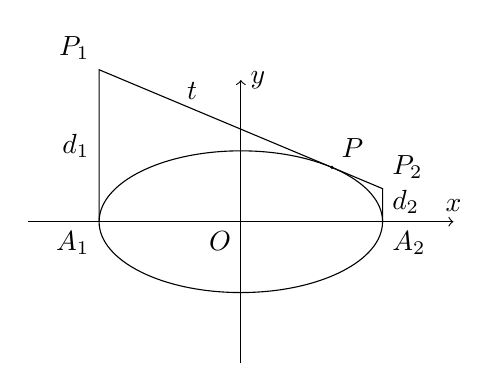
\begin{tikzpicture}[scale=0.9]
			          %projection ($(X)!(B')!(B)$)
			          %nommer chemin 'name path
			          %intersection \path [name intersections={of=d and gb,by=G}];
			          
			          %\draw[help lines] (-3,-3) grid (3,3);
			          \coordinate[label=below left:$O$](O) at (0,0);
			          \draw[->] (-3,0)--(3,0) node[above]{$x$};
				  \draw[->] (0,-2)--(0,2) node[right]{$y$};
				  \draw (0,0) ellipse (2cm and 1cm);
				  \coordinate[label=above right:$P$](P) at (1.2855,0.7666);
				  \fill (P) circle (0.025);
				  \draw (-2,0) coordinate[label=below left:$A_1$](A_1) --node[left,pos=0.5]{$d_1$} (-2,2.14437) coordinate[label=above left:$P_1$] (P_1)-- 
				  node[above,pos=0.4]{$t$}(P) -- (2,0.466338) coordinate[label=above right:$P_2$](P_2) --node[right,pos=0.4]{$d_2$} (2,0) coordinate[label=below right:$A_2$](A_2);
				  \end{tikzpicture}
				  \end{figure}
				  
				  \begin{tcolorbox}[basic] 
				      
				    \smallskip
				    \centering\underline{Procédé} \flushleft
				    Dans un repère, déterminer les coordonnées de $A_1,A_2,P_1,P_2$ pour calculer $\vect{A_1P_1}\cdot\vect{A_2P_2}$.
				    \end{tcolorbox}
		
		
		\column{.52\textwidth}\centering 
		\underline{Résolution}\\ \flushleft
		\heart Equation ellipse : $\frac{x^2}{a^2}+\frac{y^2}{b^2}=1$. \\ \medskip
		 Soit un repère orthonormé $R=(O,X,Y)$ avec : \\ \medskip
		 $A_1\ (-a,0),\ A_2\ (a,0),\ P\ (x_p,\dfrac{b}{a}\sqrt{a^2-x_p^2})$.	\\ \bigskip
		 $m(x_p) = \dfrac{b\ x_p}{a\sqrt{a^2-x_p^2}}$. \\ \bigskip
		 $t \equiv \begin{cases}
		            \ni P, \\
		            m(x_p).
		           \end{cases}\hspace{-4.5mm} \rightarrow t\equiv y=\dfrac{b(a^2-x_px)}{a\sqrt{a^2-x_p^2}}$. \\ \bigskip
		           
		$P_1(-a,\dfrac{b(a+x_p)}{\sqrt{a^2-x_p^2}}),\quad P_2(a,\dfrac{b(a-x_p)}{\sqrt{a^2-x_p^2}})$. \\ \bigskip
		
		$\vect{A_1P_1}\cdot\vect{A_2P_2} = b^2$. \hfill $\qed$

		 
		
		
		%\centering\noindent\rule{2cm}{0.4pt}
		\end{columns}
    }
	  
  
\end{document}
